
%%% Local Variables:
%%% mode: latex
%%% TeX-master: t
%%% End:

\chapter{引言}

\section{研究背景}

近年来,多核处理器已经成为主流。无论在大型服务器系统,还是在手机、平板电脑等嵌入式系统中,多核硬件都抢占了很大一部分市场。
究其原因,随着半导体制造工艺的提高,极大地缩小了CPU中基本门电路的尺寸,但同时
基于半导体技术的微电子电路已经越来越接近它的物理限制。随着这些物理限制
的临近,CPU的热功耗和数据传输同步问题已经使得通过升高单CPU主频提高系统性能的难度越来越大。尽管研究界和工业界提出了多种方法提高计算机系统的性能:如超标量流水线技术和单指令多数据流(SIMD)技术,但是Web服务器和邮件服务器一类服务器级应用更适合使用多核多进程/多线程模型提高其吞吐量。随着硬件虚拟化技术的成熟,服务器提供商可以轻易地划分单机CPU资源,进一步推动了多核CPU的普及。近年来,无论是在普通家用PC还是服务器,甚至是手机上,设备CPU核数变得越来越多已经成为了一个不可逆转的趋势。

\begin{figure}[ht]
\begin{center}
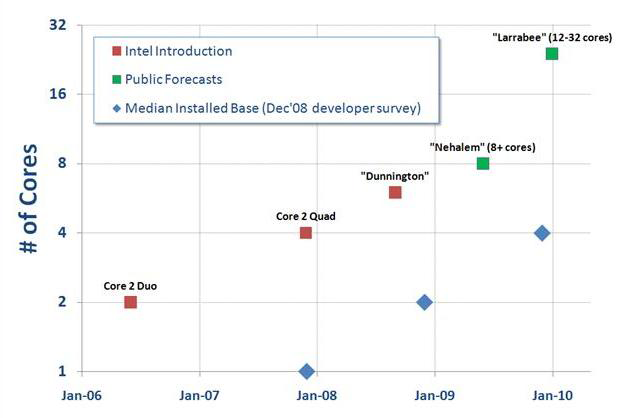
\includegraphics[width=0.7\textwidth]{figures/intro_roadmap.png}
\end{center}
\caption{Intel多核处理器发布计划图\protect\footnotemark}
\label{fig:intro_roadmap}
\end{figure}
\footnotetext{http://software.intel.com/en-us/articles/gaming-into-the-future}

在服务器应用上面,当前基于AMD64/X86\_64架构的多核系统已经得到广泛应用。但随着40核甚至
80核的NUMA系统的出现,对已有操作系统的多核可扩展性能提出了苛刻的要求。
近年越来越多的研究发现\cite{radixvm:eurosys13},由于现有操作系统在设计上的问题,OS在最新的多核系统中成为瓶颈的情况大大增多。例如,目前主流开源操作系统,如Linux和FreeBSD在应对40到80核的NUMA系统时,存在以下问题:

	\begin{itemize}
		\item
	由于已有操作系统多数是由单核系统演化而来,在设计之初就使用了一些
	不具有多核扩展性的数据结构来维护VMA、DCACHE、MountTable等内核关键
	数据结构。这导致Linux等操作系统在20核以上硬件系统上表现不佳,甚至
	出现性能下降\cite{linux:osdi10};
		\item 一些同步原语没有为重核架构优化,例如Linux的Spinlock
			实现在重核架构上导致代价高昂的Cache同步协议开销;
		\item
			操作系统设计上的问题。例如Linux中各个Core共享页表,
			在一些应用下造成不必要的TLB无效化(TLB shootdown)。
	\end{itemize}

由于现有操作系统中存在着以上这些问题,操作系统的虚拟内存管理和文件系统模块经常成为应用程序在多核系统上扩展性的瓶颈。如Exim邮件服务器、Apache
Web服务器和memcached等常用服务器应用在20核对称处理系统或NUMA系统上,常常无法无法达到与CPU核数成正比的加速比(即时在网络、磁盘等输入输出设备性能还没有达到饱和的时候仍然如此),甚至出现随着CPU核数的增加,由于操作系统内部数据竞争情况过于剧烈造成应用程序性能下降的情况\cite{linux:osdi10}。

在服务器应用以外,多核处理器已经在个人数字设备(如智能手机和平板电脑)上推广开来。2012年推出的基于ARM的NVIDIA
Tegra
3四核处理器更加明确了移动设备向多核发展的趋势。对于Linux等跨硬件平台的操作系统,如何建立更高效的多核系统抽象、设计并发友好的无锁无高速缓存竞争的数据结构变得尤为重要。

\section{课题目标}

	鉴于上述的问题,我们希望重新设计一个小型实验性操作系统和相应工具,
	从根本上解决这些问题。本毕设只考虑由于多核CPU核间通讯开销造成的操作系统性能退化,而不考虑输入输出子系统等造成的瓶颈。重头实现一个操作系统是比较有挑战性的,但我们已有uCore、MIT的xv6/SCK等实验性操作系统做参考。本课题把完成了可扩展多核操作系统实现的基础性工作,以清华大学操作系统研究组编写的uCore教学操作系统为基础,加上对AMD64
	NUMA架构的硬件抽象层(HAL)支持并在QEMU模拟器、KVM硬件虚拟化平台和基于Intel处理器的真实机器上测试通过。在此基础之上,通过模型验证和符号执行的方法,发现操作系统内部的可扩展潜能并用相关数据结构做实现。最后,完成了一种新的基于QEMU的全系统性能测试工具,帮助开发者发现系统可能存在的性能瓶颈。


